% ---------------------------------------------------------------------------
\section{\sys{}: System and Method}
\label{sec:method}

\subsection{Problem setup and agent loop}
\label{sec:setup}

An OPG $I$ is annotated as a \emph{set} of findings $F = \{f_1, \dots, f_m\}$ (possibly empty for
a healthy image), where each finding $f = (\text{quadrant}, \text{tooth position},
\text{diagnosis})$ uses FDI two-digit notation over DENTEX's four diagnosis classes
(caries, deep caries, periapical lesion, impacted tooth). The agent receives the image and a
registry of tools, and produces a sequence of turns; each turn contains free-form clinical
reasoning and zero or more structured tool calls, and the loop ends with a structured final
answer reporting \emph{every} finding the agent commits to. The same agent loop is used for
synthetic data generation, RL rollouts, and evaluation, and tool calls execute for real against
the source image at every stage (\cref{fig:pipeline}); a single shared dispatcher defines which
tools consume the image and which image they operate on, so the training and inference
environments cannot drift apart. Tool calls are capped at 50 per episode, counted by calls
rather than turns, and parsed by a bracket-counting JSON extractor that repairs truncated or
markdown-wrapped outputs.

\begin{figure}[tbp]
  \centering
  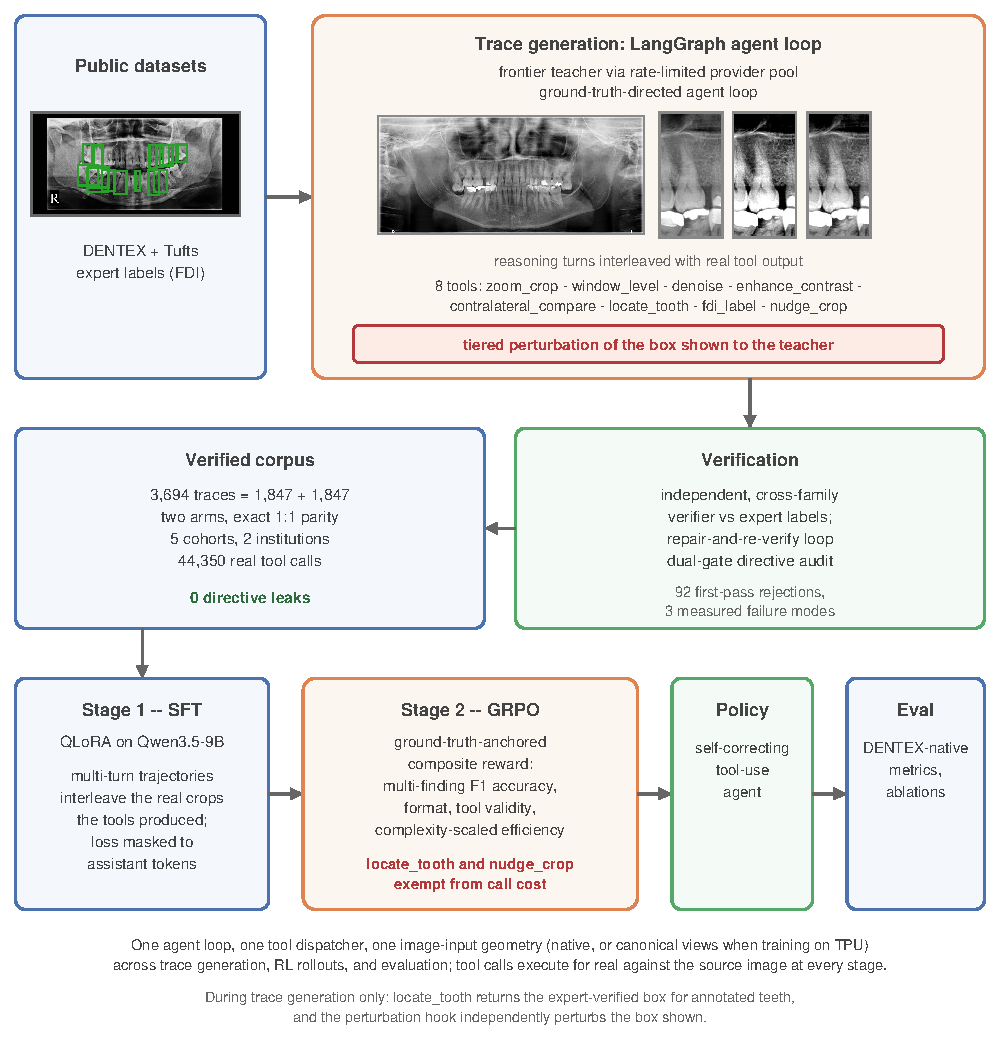
\includegraphics[width=\linewidth]{fig_pipeline}
  \caption{The \sys{} pipeline. Traces are synthesized by a frontier teacher operating a real
  tool suite in a LangGraph loop (with the tiered perturbation hook of \cref{sec:perturbation}),
  verified cross-family against expert labels, and used for SFT followed by GRPO with a
  ground-truth-anchored composite reward. Tool calls execute for real against the source image
  at every stage; the radiograph and crop pixels are real assets from the corpus (the image
  whose trace anatomy is dissected in \cref{fig:traces}).}
  \label{fig:pipeline}
\end{figure}

\subsection{System architecture}
\label{sec:architecture}

\cref{fig:architecture} shows the complete system. Five component groups surround one agent
core --- a Qwen3.5-9B vision-language policy running the loop of \cref{sec:setup}: a data layer
(\cref{fig:datasets}: registry-driven loaders for the two in-use sources, DENTEX and Tufts; a
candidate pool of eight further public panoramic datasets, promoted only after their annotation
semantics are verified; and surgical per-image Hugging Face caching), the trace
synthesis stack of \cref{sec:traces}, the two training stages of \cref{sec:reward}, and an
evaluation layer (\cref{sec:eval}) whose probes feed model selection on a fixed dev split.

\begin{figure}[tbp]
  \centering
  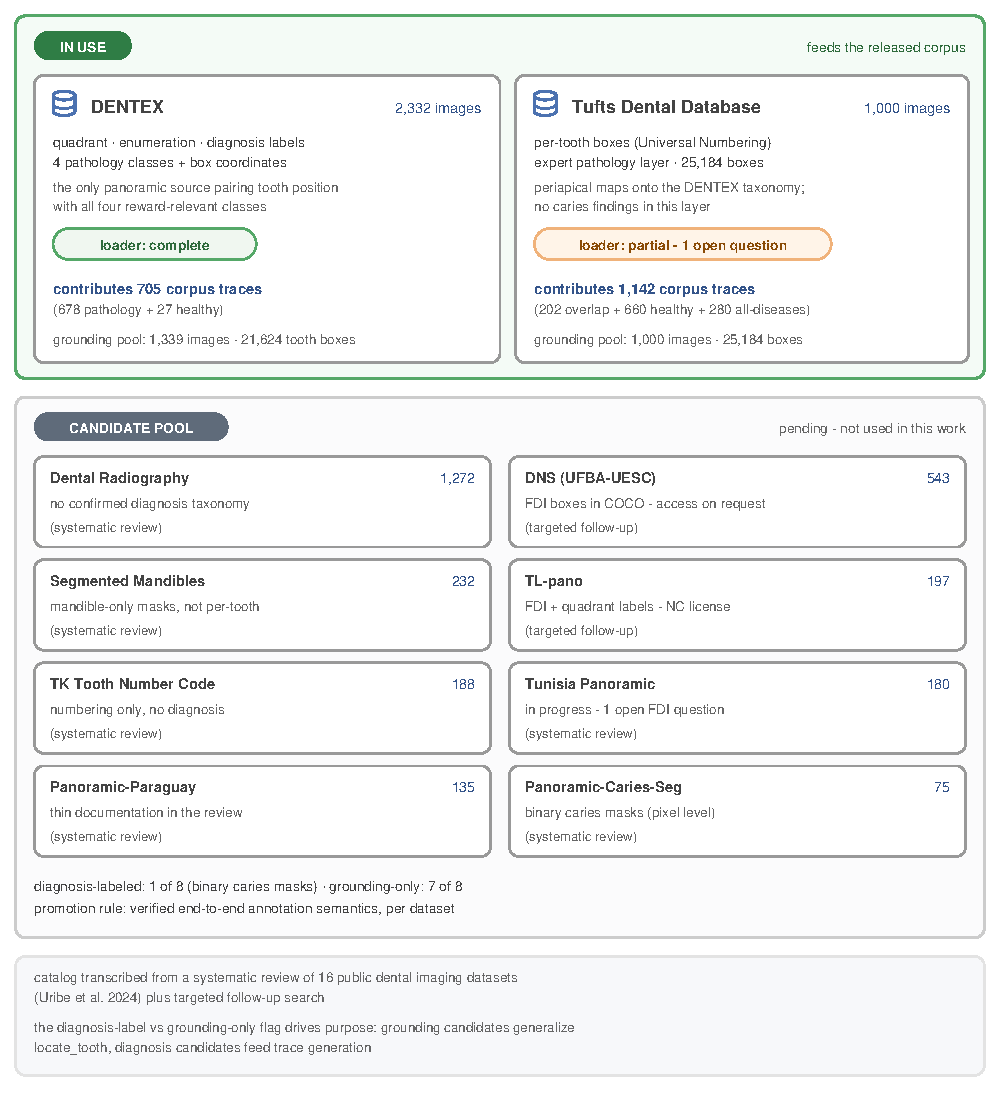
\includegraphics[width=\linewidth]{fig_datasets}
  \caption{The data layer. Two sources are in use --- DENTEX (the only panoramic dataset
  pairing tooth position with all four reward-relevant pathology classes) and the Tufts Dental
  Database (per-tooth boxes plus an expert pathology layer whose periapical class maps onto the
  DENTEX taxonomy). Eight further public panoramic datasets are catalogued as candidates and
  deliberately \emph{not} used: each would be promoted only after its annotation semantics are
  verified end-to-end, and two loaders currently stop at exactly one open question rather than
  guess. The diagnosis-label vs grounding-only flag drives purpose: grounding candidates
  generalize \texttt{locate\_tooth}, diagnosis candidates would feed trace generation.}
  \label{fig:datasets}
\end{figure}

\begin{figure}[tbp]
  \centering
  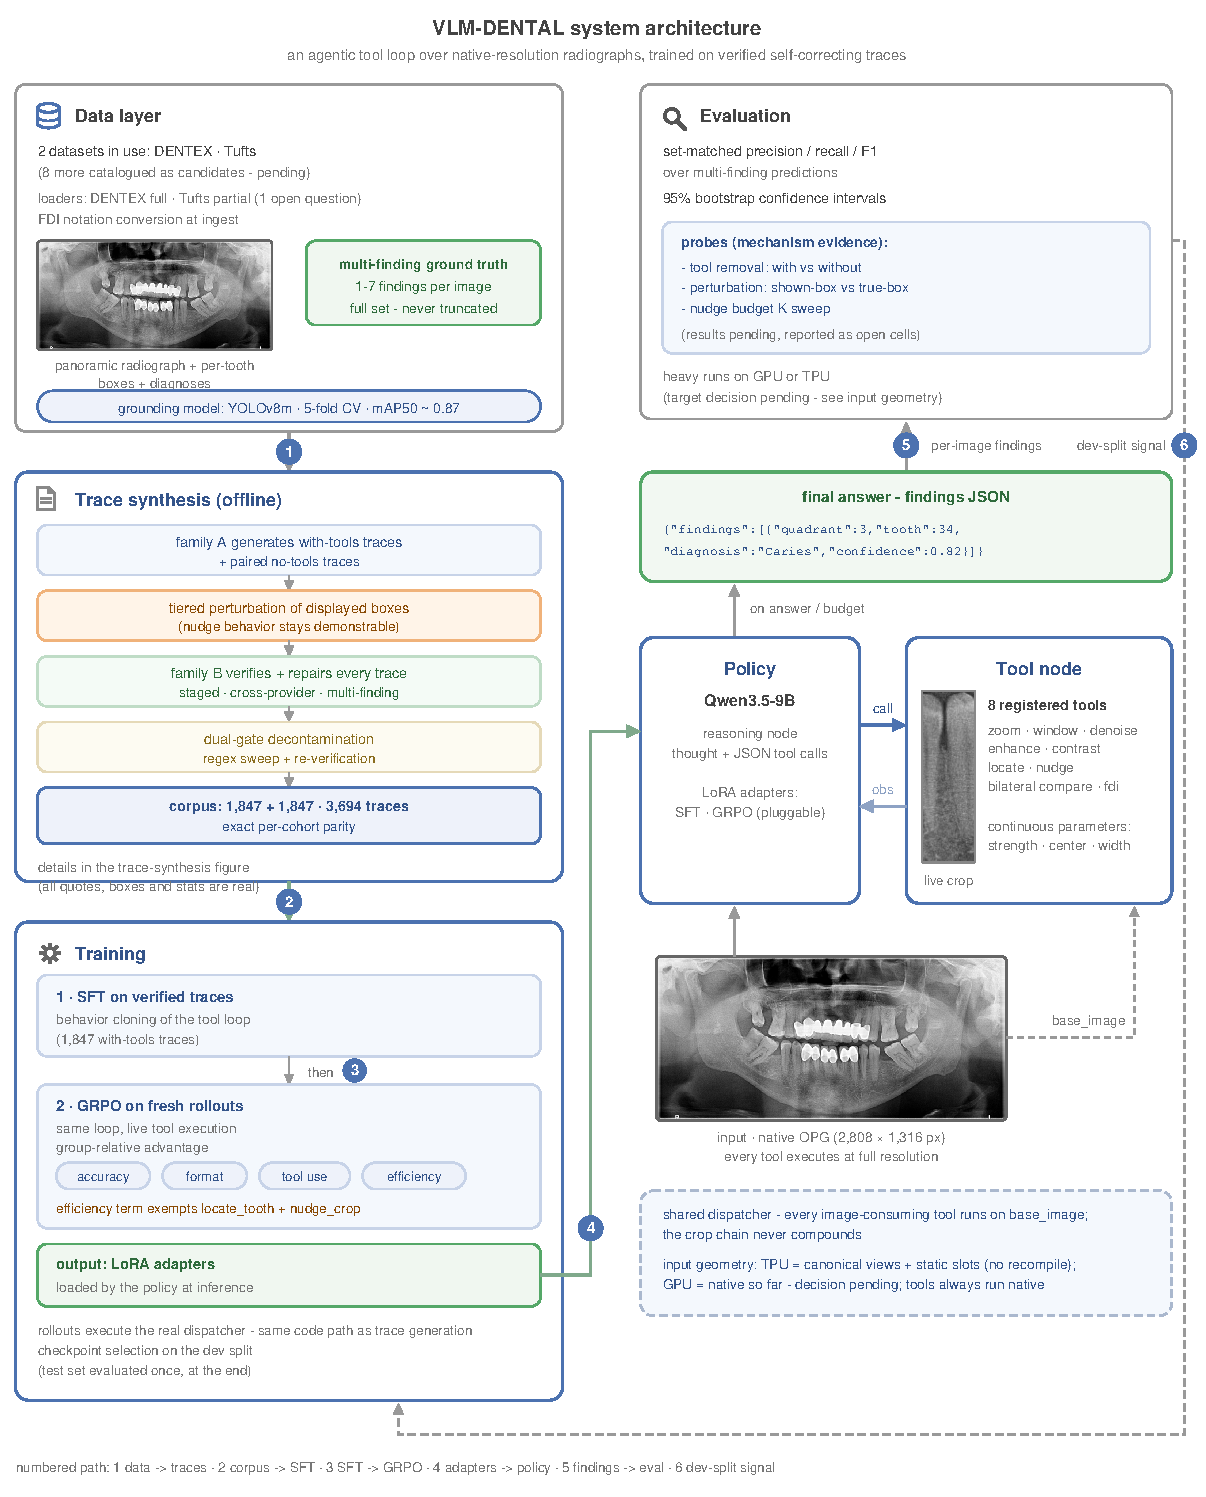
\includegraphics[width=\linewidth]{fig_architecture}
  \caption{The \sys{} architecture. One agent loop, one shared tool dispatcher, and one
  canonical vision geometry are shared by trace generation, RL rollouts, and evaluation; the
  trace synthesis stack produces the verified corpus consumed by SFT and GRPO; evaluation
  probes select on a dev split only, with the test split run once at the end. Numbered badges
  trace the corpus-to-policy life cycle (legend in the figure); radiograph and crop pixels are
  real assets from the corpus.}
  \label{fig:architecture}
\end{figure}

Three single-source-of-truth decisions hold the system together. First, one shared dispatcher
defines, for every tool, whether and \emph{which} image it consumes --- always the native source
image --- so the trace-generation loop, the GRPO rollout loop, and the evaluation runner cannot
silently diverge; the dispatcher exists precisely because the two loops originally duplicated
this logic and the rollout side drifted onto a compounding image state, a real bug that silently
invalidated rollouts. Second, the image-input geometry lives in one module and is an explicit
flag, not an implicit behavior (\cref{fig:inputgeom}). The two candidate execution targets make
different demands: TPU training requires aspect-preserving canonical views with static
vision-slot padding so XLA compiles a single graph and never recompiles, while GPU runs so far
feed original images with dynamic shapes; which target the project settles on --- a GPU
(RTX 4090 / RTX Pro 6000 / A100) or a TPU v5e-8 cluster --- is deliberately deferred to the
first GPU run. Whichever is chosen applies identically across SFT, RL, and evaluation, and in
both modes every tool operates on native-resolution pixels, so coordinates the model was trained
to emit remain valid at inference. Third, the conversion from DENTEX's zero-indexed annotation rows
to FDI notation has exactly one implementation, called by the reward, the verifier, and the
metrics alike --- an indexing bug cannot recur independently in several subsystems.

\begin{figure}[tbp]
  \centering
  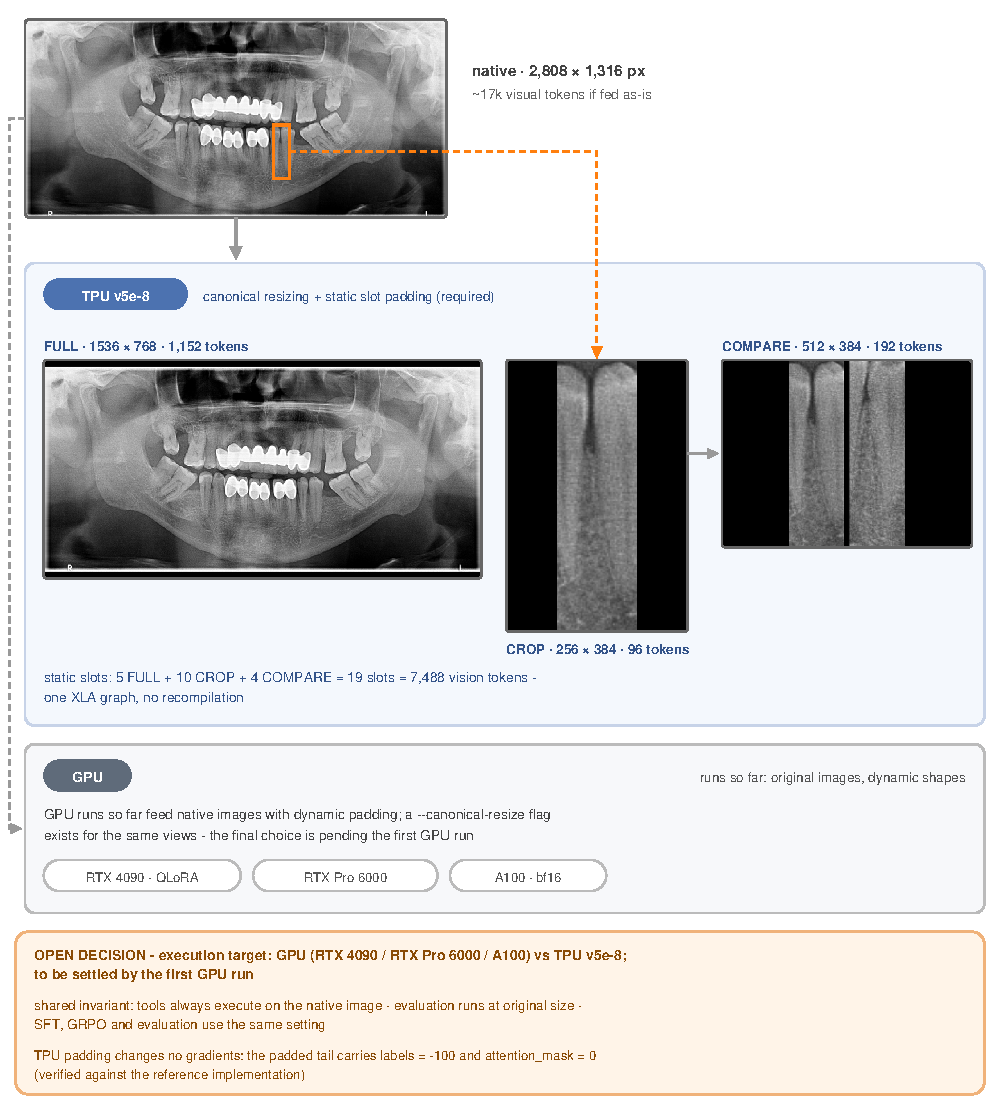
\includegraphics[width=\linewidth]{fig_input_geometry}
  \caption{Image-input geometry: two execution targets, one invariant. \textbf{TPU:} the policy
  sees aspect-preserving canonical views in three fixed families (renders produced by the
  geometry module itself, and the \texttt{contralateral\_compare} tool, from a DENTEX image),
  padded to a static 19-slot budget of 7{,}488 vision tokens so XLA compiles one graph; the
  padded tail carries $\text{labels}=-100$ and $\text{attention\_mask}=0$, so padding changes no
  gradient. \textbf{GPU:} runs so far feed original images with dynamic shapes. The choice
  between the targets is explicitly open pending the first GPU run; in both, tools always
  execute on the native image and evaluation runs at original size.}
  \label{fig:inputgeom}
\end{figure}

\subsection{A tool suite with continuous parameters}
\label{sec:tools}

The registry exposes eight tools (\cref{tab:tools}). The deliberate design choice throughout is
that tools expose \emph{how much} effect to apply as a continuous or overridable parameter, not
just a fixed on/off call: denoising takes a continuous \texttt{strength}, windowing takes exact
\texttt{center}/\texttt{width} values as an override on top of tissue presets, contrast takes a
multiplicative \texttt{factor}, and cropping takes a tunable context margin. A policy calling
\texttt{denoise(strength=0.3)} versus \texttt{denoise(strength=0.9)} is expressing a
patient-specific judgment about how grainy a crop is --- information a fixed three-level menu
cannot carry --- and the resulting tool-call stream is correspondingly more informative to train
on and to audit.

\begin{table}[tbp]
  \centering
  \small
  \caption{The \sys{} tool suite. Continuous or overridable parameters are shown in
  \emph{italics}; data-only tools return coordinates rather than images.}
  \label{tab:tools}
  \begin{tabular}{llp{6.4cm}}
    \toprule
    Tool & Key parameters & Purpose \\
    \midrule
    \texttt{zoom\_crop} & bbox, \emph{padding\_frac} & High-resolution crop of a region with a tunable context margin \\
    \texttt{window\_level} & preset; \emph{center}, \emph{width} & Radiological intensity windowing (bone/enamel/soft-tissue), exactly overridable \\
    \texttt{denoise} & method, \emph{strength} $\in[0,1]$ & Edge-preserving bilateral or median filtering matched to crop noise \\
    \texttt{enhance\_contrast} & \emph{factor} & Multiplicative contrast adjustment for subtle lesions \\
    \texttt{contralateral\_compare} & bbox, quadrant & Side-by-side mirror crop, constrained to the correct jaw half, for bilateral symmetry assessment \\
    \texttt{locate\_tooth} & FDI tooth & YOLOv8m grounding (32 classes, one per FDI position); returns a box \\
    \texttt{fdi\_label} & quadrant, position & FDI notation conversion and validation \\
    \texttt{nudge\_crop} & bbox, \emph{dx\_frac}, \emph{dy\_frac}, \emph{scale} & Correct a box the agent was already given, without re-running detection \\
    \bottomrule
  \end{tabular}
\end{table}

\subsection{Self-correcting grounding: \texttt{nudge\_crop}}
\label{sec:nudge}

The grounding tool is a YOLOv8m detector fine-tuned on 2{,}339 DENTEX+Tufts images with 46{,}808
tooth boxes, trained with 5-fold cross-validation (one class per FDI quadrant--position pair)
(\cref{fig:groundingcv}; full per-fold numbers in \cref{app:grounding}).
It is strong --- held-out \emph{target} mAP50 of 0.93--0.96 with precision up to 0.986 on
annotated teeth --- but it is a 32-class detector operating under per-fold variance, and its
errors are exactly the kind that poison downstream reasoning: a box shifted by half a
tooth-width produces a crop that still \emph{looks} like a plausible anatomical region while
showing the wrong tooth.

\begin{figure}[tbp]
  \centering
  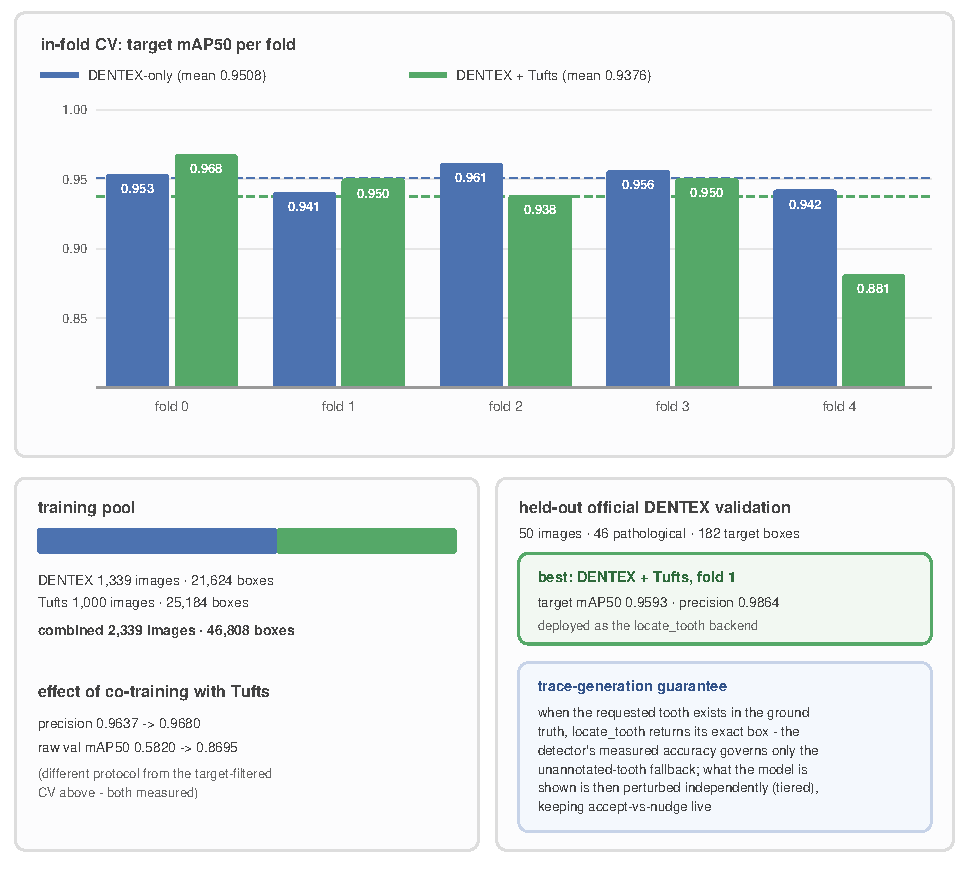
\includegraphics[width=\linewidth]{fig_grounding_cv}
  \caption{The \texttt{locate\_tooth} backend: YOLOv8m trained with 5-fold cross-validation on
  the combined DENTEX+Tufts pool (2{,}339 images, 46{,}808 tooth boxes). Left: in-fold
  target mAP50 per fold for the DENTEX-only and multi-dataset models (means 0.9508 / 0.9376).
  Right: pool composition, the held-out official DENTEX validation (best target mAP50 0.9593 at
  precision 0.9864 --- the deployed checkpoint), and the trace-generation guarantee: when a
  requested tooth exists in the ground truth, \texttt{locate\_tooth} returns its exact box, and
  only the \emph{displayed} copy is perturbed. Exact per-fold numbers in \cref{app:grounding}.}
  \label{fig:groundingcv}
\end{figure}

\texttt{nudge\_crop} turns that failure mode into an interaction. It takes a box the policy was
\emph{already given} (by \texttt{locate\_tooth} or a previous \texttt{nudge\_crop} --- never
asserted from nowhere) and returns adjusted coordinates: a shift $(\texttt{dx\_frac},
\texttt{dy\_frac})$ expressed as fractions of the box's own width and height, and a rescale
\texttt{scale} around the new center, clamped to image bounds. The tool is deliberately
\emph{data-only}: it computes coordinates, and the policy must pair it with \texttt{zoom\_crop}
to actually see the corrected region. Two consequences follow. First, the fractional,
box-relative parameterization is what a VLM can reason about reliably --- ``shift left by about
half the box'' --- rather than raw pixel coordinates at an arbitrary zoom level. Second, because
each correction must be followed by a verification crop, the loop enforces an
inspect--correct--re-inspect cycle rather than a single blind adjustment. This is the mechanism
neither concurrent dental agentic system provides: their tools are fixed operations whose
outputs the policy can only accept.

\subsection{Tiered perturbation: making self-correction learnable}
\label{sec:perturbation}

A policy can only learn to interrogate its tools if its teachers did. The core difficulty is
that an idealized demonstrator --- one whose grounding tool always returns the right box ---
demonstrates \emph{trusting} the tool, and SFT on such traces teaches exactly the wrong
reflex. At the same time, blind exploration by the demonstrator would collapse the yield of
usable traces.

Our resolution (\cref{fig:mechanism}) separates what the grounding tool \emph{computes} from
what the demonstrator \emph{sees}. During trace generation, \texttt{locate\_tooth} operates in a
ground-truth-grounding mode: for an annotated tooth it returns the expert-verified box
(guaranteeing the demonstration remains solvable), while for exploratory calls on unannotated
teeth it falls back to real detector inference. Then, independently of how the box was obtained,
a \emph{perturbation roll} decides what is displayed:

\begin{itemize}[leftmargin=*,itemsep=1pt,topsep=2pt]
  \item \textbf{none} (45\%): the box is shown as computed --- a clean accept-and-proceed demonstration;
  \item \textbf{small} (25\%): a synthetic offset of 12--28\% of the box's own size per axis,
  random sign --- a genuine judgment call that the zoom margin often absorbs, and that the prompt
  deliberately does \emph{not} resolve either way;
  \item \textbf{big} (30\%): an offset of 45--75\% per axis --- sized to be visually self-evident.
\end{itemize}

Offsets are applied with \texttt{nudge\_crop}'s own shift-and-clamp math, so every perturbed box
is one the correction tool could plausibly have produced or fixed; the unperturbed box is logged
internally for auditing but never shown. Two design commitments matter more than the numbers:

\paragraph{Fixed rates, decoupled from detector accuracy.}
The perturbation probabilities are configured constants, not a reflection of the grounding
model's measured error rate. This is a deliberate decoupling: if ``how often the model must
verify'' tracked the detector's live precision, then every improvement to the detector would
silently reduce the frequency of demonstrated correction, and traces generated under the old
detector would teach a stale behavior. With fixed rates, today's corpus remains valid as the
grounding tool improves --- a property this project exercised for real, as the detector's
validated mAP50 improved from 0.58 (DENTEX-only) to 0.87--0.96 (multi-dataset) while the trace
corpus stayed in use unchanged.

\paragraph{No verbal cue; magnitude carries the signal.}
Nothing in the trace-generation prompt marks a perturbed box as wrong. A verbal cue (``this box
needs correction'') would exist only during data generation and not at RL or inference time, so
teaching the model to respond to it would be a shortcut that fails exactly when it matters. The
big tier is therefore sized to be self-evident from the crop alone, and the small tier is left
genuinely ambiguous --- the demonstrator has to look and judge, which is precisely the skill the
deployed policy must exercise with no ground truth available at all.

\begin{figure}[tbp]
  \centering
  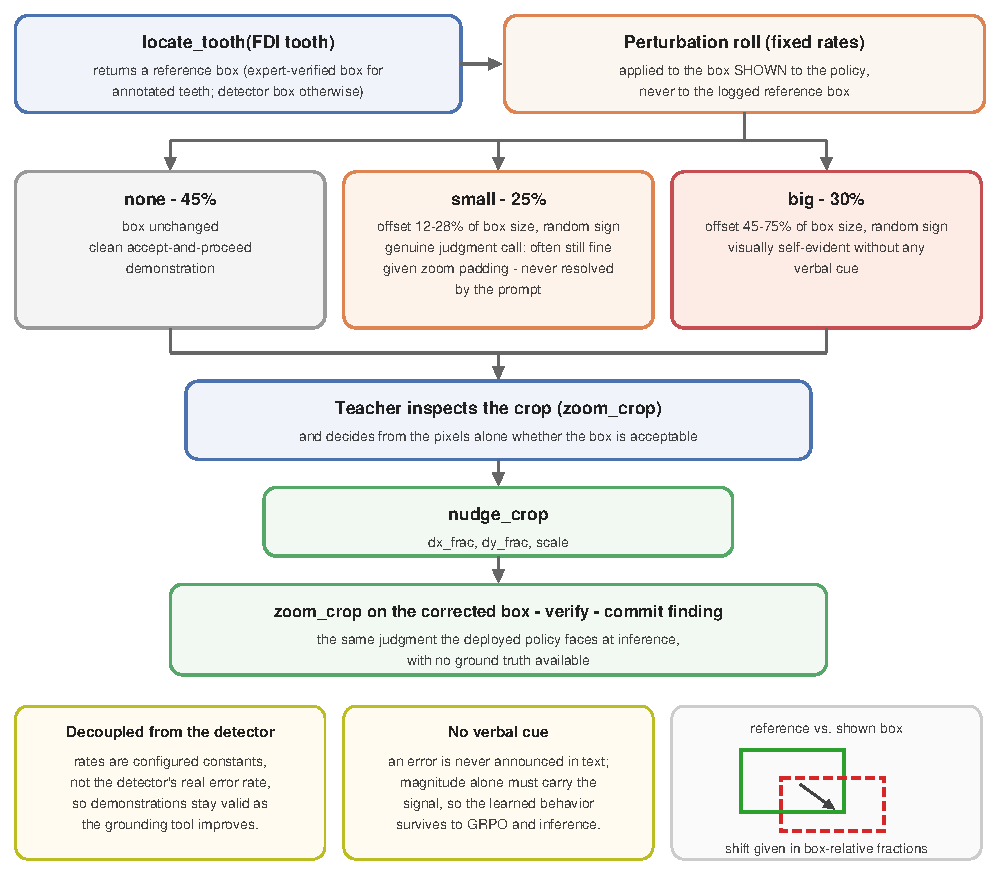
\includegraphics[width=\linewidth]{fig_perturbation_mechanism}
  \caption{The tiered perturbation mechanism and the correction loop it trains. The perturbation
  applies to the box shown to the policy only; offsets reuse \texttt{nudge\_crop}'s own math; and
  no verbal cue marks an error, so the offset magnitude alone must carry the signal.}
  \label{fig:mechanism}
\end{figure}

\subsection{Trace generation, verification, and decontamination}
\label{sec:traces}

Traces are generated by a frontier teacher (Gemini 3.5 Flash Lite or MiniMax M3, routed through
a rate-limited provider pool) that is directed toward the expert labels for the image but writes
its own reasoning and tool calls turn by turn under real tool feedback. Generation is
ground-truth-directed by design: blind exploration by an untuned model would tank the yield of
correctly-labeled demonstrations. Every trace then passes an independent, cross-family
\emph{verifier} conditioned on the image and the expert labels, which rejects reasoning not
supported by what the model was actually shown. Verification is staged rather than monolithic
(\cref{fig:multistage}): a strict pass checks diagnostic correctness, FDI validity, and whether
every claim is supported by what the model was actually shown --- treating valid
\texttt{nudge\_crop} correction loops as evidence of diligence rather than as errors --- and
rejected traces are routed to a verifier-editor that surgically repairs FDI labels, diagnosis
labels, and formatting while preserving the clinical chain of thought; the repaired trace is
re-verified before promotion. Both stages are cross-family by construction: the generator and
the verifier are routed through separate provider pools spanning different model families
(Gemini, MiniMax, NVIDIA NIM, Groq, OpenRouter), so a generator's blind spot is unlikely to be
shared by its judge. Because generation is conditioned on privileged information, traces are
scanned for \emph{directive leakage} --- the demonstrator echoing its hidden instructions in its
reasoning --- and leaking cases are excised and regenerated under a dual gate (zero-leak regex
audit + verifier re-approval); the canonical corpus contains zero leaks.

\begin{figure}[tbp]
  \centering
  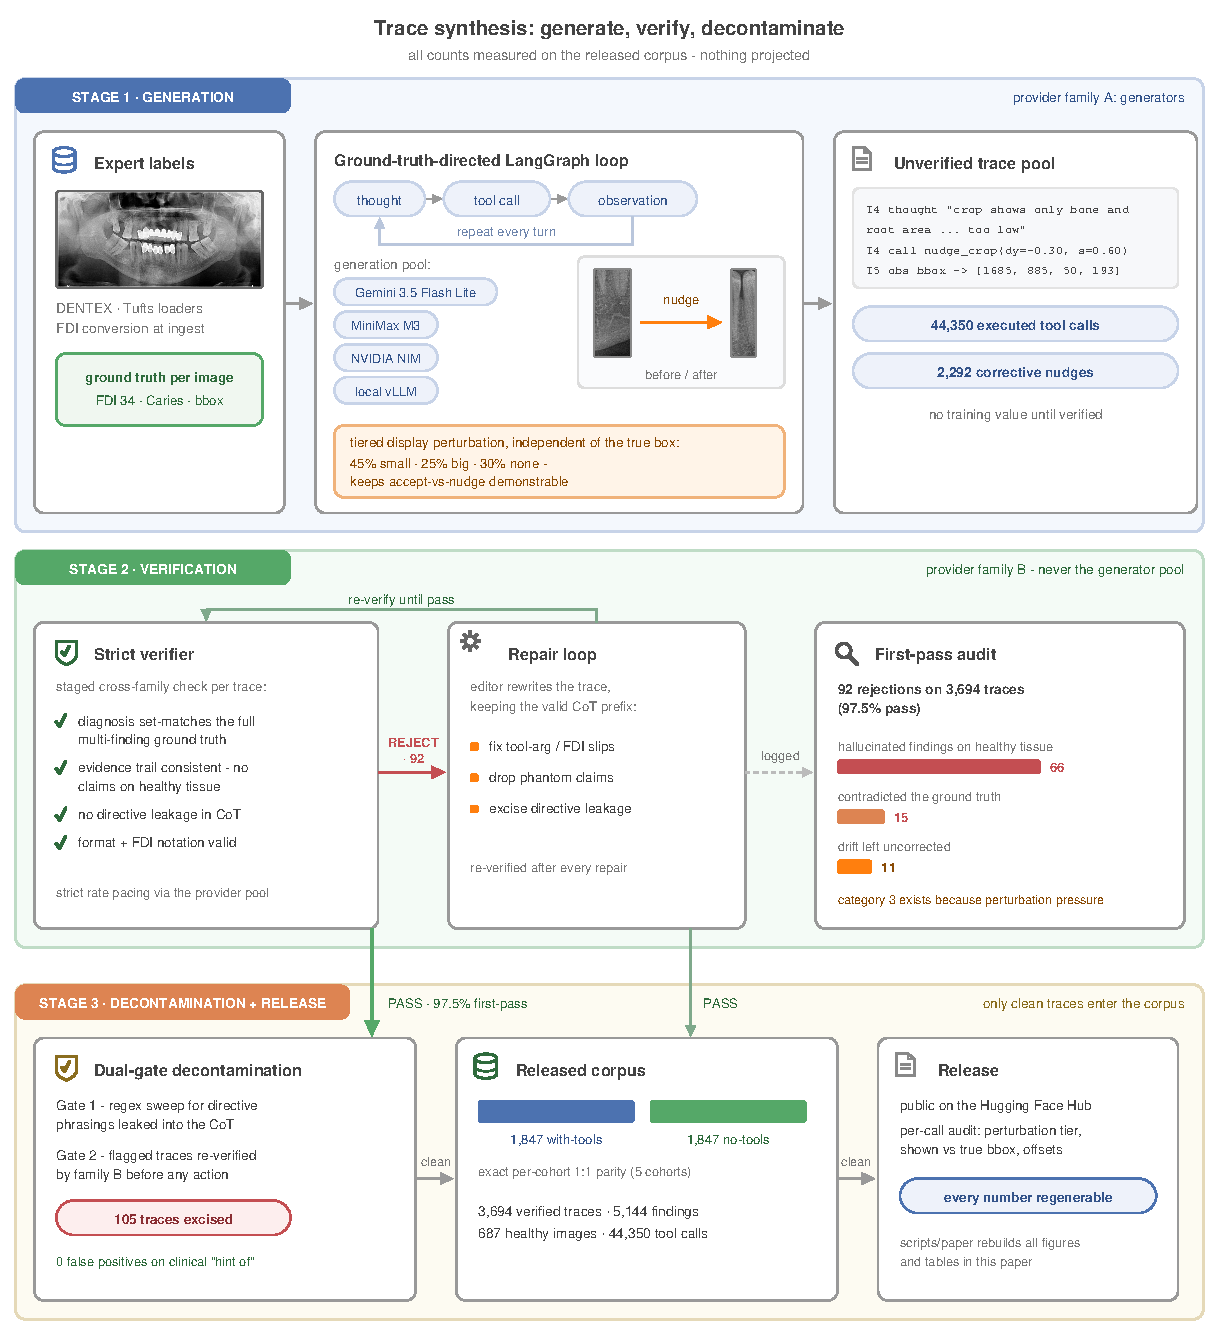
\includegraphics[width=0.92\linewidth]{fig_trace_multistage}
  \caption{Multi-stage trace synthesis. Generation (provider family A) runs a
  ground-truth-directed LangGraph loop with real tool execution and the tiered perturbation
  hook; staged verification (deliberately a \emph{different} provider family) combines a strict
  clinical pass with a repair-and-re-verify loop; a dual-gate leak audit and corpus assembly
  produce the frozen canonical release; the audit bars are measured counts. The verifier's
  92 first-pass rejections span three
  categories --- the third (uncorrected spatial drift) exists only because the perturbation
  mechanism creates genuine judgment pressure.}
  \label{fig:multistage}
\end{figure}

\begin{figure}[tbp]
  \centering
  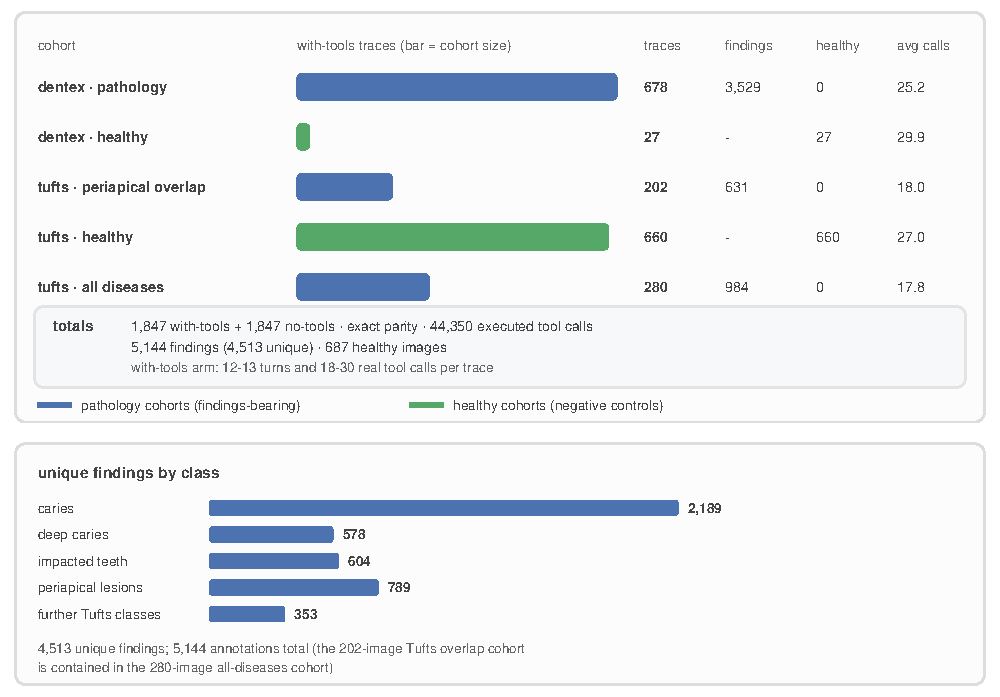
\includegraphics[width=\linewidth]{fig_corpus_composition}
  \caption{Corpus composition (measured from the released trace files). Five cohorts --- three
  findings-bearing, two healthy negative controls --- exist in two exact arms (with-tools and
  no-tools) with per-cohort 1:1 parity; the with-tools corpus carries 5{,}144 finding-level
  annotations (4{,}513 unique: the 202-image Tufts overlap cohort is contained in the 280-image
  Tufts all-diseases cohort, so its findings are counted in both). Class mix of the unique
  findings below; the teacher surveys every finding on an image, and healthy scans carry empty
  finding sets.}
  \label{fig:corpus}
\end{figure}

The resulting corpus (\cref{tab:corpus}, \cref{fig:corpus}) comprises 3{,}694 verified traces over 1{,}847 images
from two institutions: 1{,}847 interactive with-tools traces and 1{,}847 single-turn no-tools
traces in exact 1:1 parity --- the paired design that lets the evaluation isolate the
contribution of the tools (\cref{sec:eval}). The with-tools corpus carries 5{,}144
finding-level ground-truth annotations across cohorts (4{,}513 unique: the 202-image Tufts
overlap cohort is contained in the 280-image Tufts all-diseases cohort, so its 631 findings are
counted twice), spanning caries (2{,}189), deep caries (578), impacted teeth (604), periapical
lesions (789 unique), and three further Tufts lesion classes (353); multi-finding images carry
up to 23 annotated findings, and the teacher surveys every finding on the image. Healthy scans
are included as negative controls with empty finding sets. The verifier rejected 92 traces
across three failure modes: 66 hallucinated findings on healthy scans, 15 ground-truth
contradictions (wrong diagnosis class or swapped quadrants), and 11 uncorrected spatial drifts
--- cases where the teacher diagnosed from a visibly displaced box without issuing a corrective
\texttt{nudge\_crop}. The third category is direct evidence that the perturbation mechanism
creates real, auditable judgment pressure rather than a scripted step. Across the with-tools
corpus the teacher averaged 12--13 turns and 18--30 real tool calls per trace
(\cref{tab:corpus}); the full call distribution is shown in \cref{fig:toolusage}.

\begin{table}[tbp]
  \centering
  \small
  \caption{The verified corpus, regenerated from the released trace files. With-tools and
  no-tools cohorts are in exact 1:1 parity (checkmarks). Turns and tool calls are for the
  with-tools side; findings are counted per cohort (the Tufts overlap cohort is a subset of the
  Tufts all-diseases cohort, so its findings are counted in both).}
  \label{tab:corpus}
  \begin{tabular}{lrrrrrr}
\toprule
Cohort & With-tools & No-tools & Findings & Healthy & Turns & Tool calls \\
\midrule
DENTEX pathology & 678 & 678~\checkmark & 3529 & 0 & 12.9 & 25.2 \\
DENTEX healthy (negative controls) & 27 & 27~\checkmark & 0 & 27 & 13.4 & 29.9 \\
Tufts overlap pathology & 202 & 202~\checkmark & 631 & 0 & 12.0 & 18.0 \\
Tufts healthy (negative controls) & 660 & 660~\checkmark & 0 & 660 & 12.8 & 27.0 \\
Tufts 4-disease pathology & 280 & 280~\checkmark & 984 & 0 & 11.7 & 17.8 \\
\midrule
Total & 1847 & 1847~\checkmark & 5144 & 687 & -- & -- \\
\bottomrule
\end{tabular}
\end{table}

\begin{figure}[tbp]
  \centering
  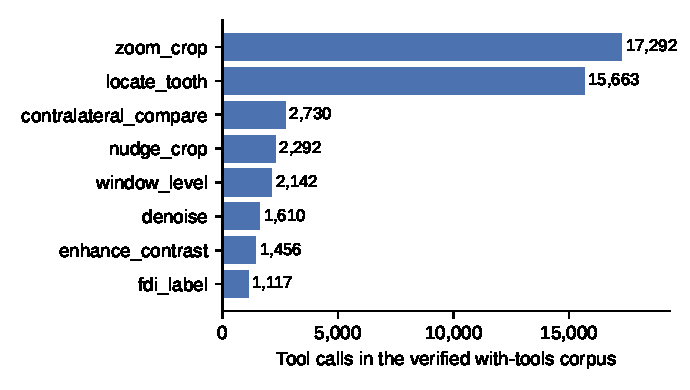
\includegraphics[width=0.62\linewidth]{fig_tool_usage}
  \caption{Recorded tool-call attempts over the verified with-tools corpus (44{,}350 across
  1{,}847 traces, of which 48 were invalid --- e.g.\ a hallucinated \texttt{localize\_tooth} ---
  and returned a standard error observation to the agent).
  \texttt{zoom\_crop} and \texttt{locate\_tooth} dominate;
  \texttt{nudge\_crop} appears 2{,}292 times as genuine mid-episode correction.}
  \label{fig:toolusage}
\end{figure}

\subsection{Anatomy of a trace: with tools vs.\ without}
\label{sec:traceanatomy}

\cref{fig:traces} shows both halves of the paired corpus for one DENTEX image (a carious FDI
tooth 34, a single finding). The no-tools trace is one turn: a fluent, well-structured direct
diagnosis that happens to reach the right answer, with no evidence trail --- the reasoning
cannot be checked against anything the model was actually shown, and the model never had the
opportunity to be wrong and recover. The with-tools trace for the same image runs 23 turns and
22 real tool calls and demonstrates the full behavioral repertoire the perturbation mechanism is
designed to elicit: the grounding box for tooth 34 was inspected, judged wrong (``the crop shows
only bone/root area \ldots the box appears to be too low''), and corrected three times with
box-relative \texttt{nudge\_crop} shifts until re-inspection confirmed the crown; a
contralateral symmetry comparison and a contrast-enhanced re-inspection followed before the
structured final answer, which matches the expert label.

\begin{figure}[tbp]
  \centering
  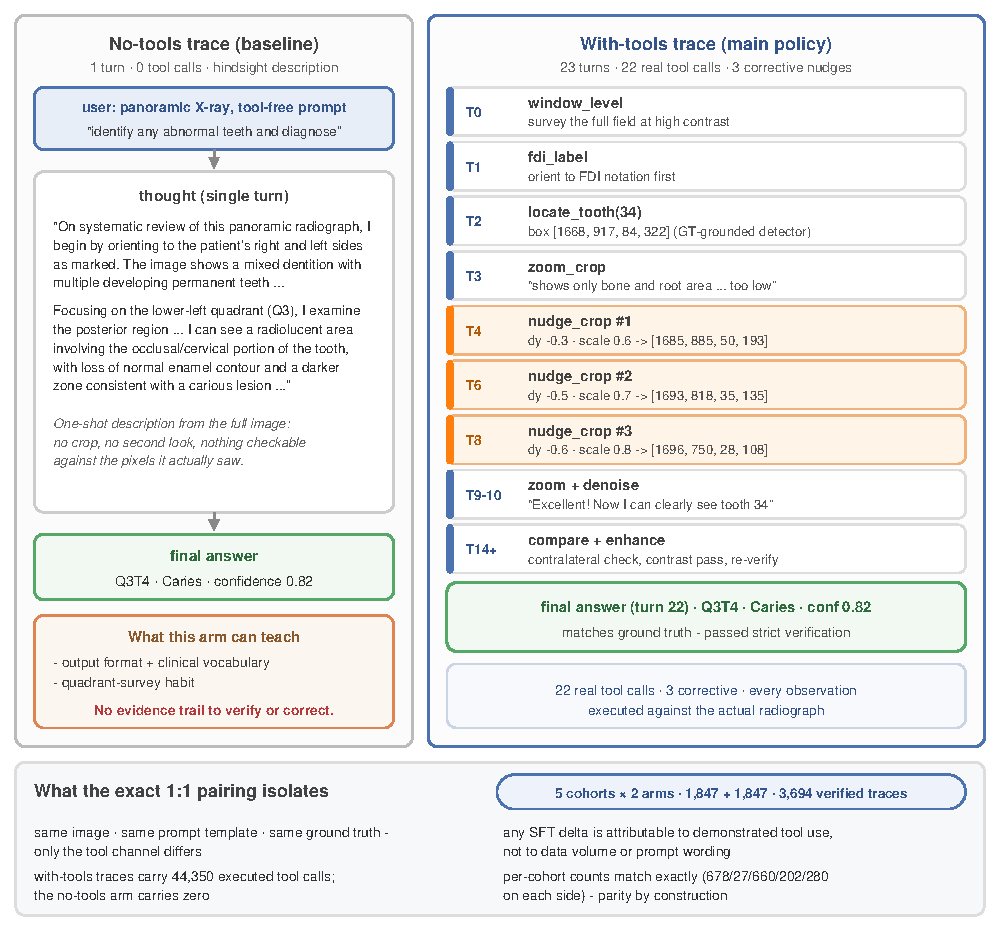
\includegraphics[width=0.88\linewidth]{fig_traces_comparison}
  \caption{Two training traces for the same image (DENTEX, carious FDI 34) and the same expert
  label. Left: the real radiograph with the with-tools evidence trail --- the returned grounding
  box (blue), the three corrective \texttt{nudge\_crop} boxes (orange, light to dark, magnified
  in the inset; the arrow marks the upward walk from the returned box to the corrected one),
  and the expert box (green dashed); all coordinates are the
  values actually returned by the tools, and the right panel shows the crop the teacher finally
  saw. Middle: the single-turn no-tools trace --- fluent, correct, and unverifiable. Right: the
  with-tools trace (23 turns, 22 real tool calls), in which the grounding box is inspected,
  judged wrong, corrected three times, and re-inspected before the answer; quotes are abridged
  from the released traces. The two arms exist in exact per-cohort 1:1 parity, so the evaluation
  can vary only the tool interface.}
  \label{fig:traces}
\end{figure}

The paired design is what makes this contrast usable rather than anecdotal. With 1{,}847
with-tools and 1{,}847 no-tools traces in exact per-cohort parity, the evaluation can hold the
image and the label fixed and vary only the tool interface, isolating what interactive tool use
adds over single-pass reasoning (\cref{sec:eval}). The no-tools traces are retained
deliberately: they teach output format and clinical vocabulary and provide the baseline arm of
every comparison --- but they are documented as ground-truth-directed single-pass generation
(closer to hindsight rationalization than blind discovery), a tradeoff \cref{sec:traces} made
explicit rather than hidden.

\subsection{Training: SFT then GRPO with a correction-friendly reward}
\label{sec:reward}

Stage 1 (SFT) fine-tunes Qwen3.5-9B \citep{bai2025qwen25vl} with QLoRA \citep{dettmers2023qlora}
on the verified with-tools traces, teaching the \emph{shape} of the behavior: well-formed
reasoning, well-formed tool calls with continuous parameters, and structured multi-finding final
answers. Multi-turn trajectories interleave the real crops the tools produced, and loss is
masked to assistant tokens only.

Stage 2 (GRPO \citep{deepseek2025r1}) optimizes the composite reward
\[
  R = w_{\text{acc}} R_{\text{acc}} + w_{\text{fmt}} R_{\text{fmt}}
    + w_{\text{tool}} R_{\text{tool}} + w_{\text{eff}} R_{\text{eff}},
\]
with three properties that matter for this task:

\paragraph{Ground-truth-anchored, multi-finding accuracy.}
$R_{\text{acc}}$ is a hard, non-LLM-judge match against expert labels. Predicted findings are
matched to annotated findings one-to-one by greedy highest-score-first assignment; each matched
pair scores $0.25 \cdot
\mathbf{1}[\text{quadrant}] + 0.25 \cdot \mathbf{1}[\text{position}] + 0.50 \cdot
\mathbf{1}[\text{diagnosis}]$, and the image-level score is the F1-style harmonic mean of the
matched recall and precision --- missed findings and hallucinated extra findings both score
zero, so spamming guesses cannot free-ride. With one finding on each side this reduces exactly
to the single-pair score. This design follows \citet{oralgptplus2026}'s documented
reward-hacking failure under an LLM-judge accuracy term: our accuracy signal is not a judge's
opinion and cannot be collapsed by calling one tool and stopping.

\paragraph{Complexity-scaled efficiency that does not fight correction.}
A naive per-call penalty prices every tool call equally --- and therefore prices a legitimate
corrective \texttt{nudge\_crop} the same as aimless spam, directly fighting the behavior
\cref{sec:perturbation} exists to teach. $R_{\text{eff}}$ instead derives a reference budget
from the trajectory itself (6 calls per distinct located tooth), exempts \texttt{locate\_tooth}
and \texttt{nudge\_crop} entirely from per-call cost, and charges only budget overruns and
exact back-to-back repeat calls (which yield no new information), with a smooth drop-off rather
than a hard cliff.

\paragraph{Dual-adapter RL.}
The frozen SFT adapter serves as the KL reference policy on the same base model, computing the
KL penalty by adapter swapping rather than a second model in memory.
